% M4 σύντομη παρουσίαση — LaTeX Beamer, widescreen 16:9 (όπως PowerPoint).
% Compile:  lualatex M4_parousiasi.tex   (χρειάζεται fontspec/polyglossia για ελληνικά)
\documentclass[aspectratio=169,12pt]{beamer}

\usepackage{fontspec}
\usepackage{polyglossia}
\setmainlanguage{greek}
\setotherlanguage{english}

% Explicit Windows font paths so fontspec/luaotfload doesn't need a font-db rebuild.
\setmainfont{Arial}[
  Path = C:/Windows/Fonts/,
  Extension = .ttf,
  UprightFont = arial,
  BoldFont = arialbd,
  ItalicFont = ariali,
  BoldItalicFont = arialbi
]
% Beamer's default text family is SANS, not roman -- polyglossia checks that
% family for Greek glyph support too, so it must be set explicitly as well.
\setsansfont{Arial}[
  Path = C:/Windows/Fonts/,
  Extension = .ttf,
  UprightFont = arial,
  BoldFont = arialbd,
  ItalicFont = ariali,
  BoldItalicFont = arialbi
]
\renewcommand{\familydefault}{\sfdefault}
\newfontfamily\greekfont{Arial}[
  Path = C:/Windows/Fonts/,
  Extension = .ttf,
  UprightFont = arial,
  BoldFont = arialbd,
  ItalicFont = ariali,
  BoldItalicFont = arialbi
]
\newfontfamily\greekfontsf{Arial}[
  Path = C:/Windows/Fonts/,
  Extension = .ttf,
  UprightFont = arial,
  BoldFont = arialbd,
  ItalicFont = ariali,
  BoldItalicFont = arialbi
]
\newfontfamily\headfont{Cambria}[
  Path = C:/Windows/Fonts/,
  UprightFont = {cambria.ttc},
  BoldFont = {cambriab.ttf},
  ItalicFont = {cambriai.ttf},
  BoldItalicFont = {cambriaz.ttf}
]

\usepackage{tikz}
\usetikzlibrary{shapes.geometric,positioning,calc,arrows.meta}
\usepackage{graphicx}
\usepackage{array}

% ---- palette: "Midnight Executive" (navy / ice-blue) + green=success, red=fail, gold=accent ----
\definecolor{navy}{HTML}{152238}
\definecolor{navytwo}{HTML}{1E3A5F}
\definecolor{ice}{HTML}{EAF2FA}
\definecolor{txtcol}{HTML}{1B2233}
\definecolor{mutedcol}{HTML}{5B6B82}
\definecolor{greencol}{HTML}{1E8F5F}
\definecolor{redcol}{HTML}{B23A2E}
\definecolor{goldcol}{HTML}{D8A93A}

\setbeamertemplate{navigation symbols}{}
\setbeamercolor{background canvas}{bg=white}
\setbeamercolor{normal text}{fg=txtcol}
\setbeamercolor{frametitle}{fg=txtcol,bg=white}
\setbeamerfont{frametitle}{family=\headfont,series=\bfseries,size=\Large}
\setbeamertemplate{frametitle}{\vspace{4mm}\insertframetitle\vspace{2mm}}
\setbeamertemplate{footline}{}
\setbeamertemplate{itemize items}[circle]
\setbeamercolor{itemize item}{fg=navy}

\newcommand{\cardtitle}[1]{{\headfont\bfseries\large #1}}

\title{}
\author{}
\date{}

\begin{document}

% ===================================================================
% 1. Τίτλος
% ===================================================================
\begin{frame}[plain]
\begin{tikzpicture}[remember picture,overlay]
  \fill[navy] (current page.south west) rectangle (current page.north east);
  \fill[navytwo] ($(current page.north east)+(-2.1,-0.9)$) circle (1.05);
  \fill[goldcol,opacity=0.30] ($(current page.north east)+(-1.15,-1.95)$) circle (0.65);
  \fill[navytwo] ($(current page.south west)+(0.95,1.1)$) circle (0.8);

  % anchor=north west so multi-line blocks stack top-down predictably (a
  % vertically-centered "west" anchor made the 2-line title's true bottom
  % edge land lower than expected and collide with the subtitle below it).
  \node[anchor=north west,text width=11.6cm,align=left] at ($(current page.west)+(1.0,2.1)$)
    {\headfont\bfseries\fontsize{26}{30}\selectfont\color{white}
     Νευρομορφική Ρομποτική\\ Πλοήγηση};
  \node[anchor=north west,text width=11.6cm,align=left] at ($(current page.west)+(1.0,-0.35)$)
    {\fontsize{13}{16}\selectfont\color{ice}
     Spiking Neural Network με R-STDP πλαστικότητα\ \ $\cdot$\ \ Go2 quadruped\ \ $\cdot$\ \ FPGA-inspired υλικό};
  \node[anchor=north west,text width=11.6cm,align=left] at ($(current page.west)+(1.0,-1.65)$)
    {\fontsize{12}{15}\selectfont\itshape\color{goldcol}
     Πειραματική επίδειξη M4 — το πρώτο θετικό σήμα ανάκαμψης};
  \node[anchor=west] at ($(current page.south west)+(1.0,0.6)$)
    {\fontsize{9}{11}\selectfont\color{mutedcol!80!white} Προπτυχιακή Διπλωματική \ $\cdot$\ ΗΜΜΥ};
\end{tikzpicture}
\end{frame}

% ===================================================================
% 2. Το ερώτημα
% ===================================================================
\begin{frame}{Το ερώτημα}
\begin{columns}[T,totalwidth=\textwidth]
\begin{column}{0.46\textwidth}
\begin{tikzpicture}
  \node[fill=navy,rounded corners=6pt,text width=6.6cm,minimum height=6.9cm,
        inner sep=10pt,align=left,anchor=north west] (box) at (0,0) {};
  \node[anchor=north west,text width=6.2cm,align=left] at ($(box.north west)+(0.25,-0.25)$)
    {\headfont\bfseries\fontsize{22}{22}\selectfont\color{goldcol} H1};
  \node[anchor=north west,text width=6.1cm,align=left] at ($(box.north west)+(0.25,-1.15)$)
    {\fontsize{11.5}{15}\selectfont\color{ice}
     Ανακάμπτει ένα SNN με online R-STDP πλαστικότητα πιο γρήγορα/καλύτερα από ένα
     \textbf{\color{goldcol}παγωμένο} δίκτυο, όταν αλλάζει κάτι στη μέση της αποστολής;};
\end{tikzpicture}
\end{column}
\begin{column}{0.5\textwidth}
  \vspace{-2mm}
  {\small
  \textbf{Ρομπότ} \\[-1pt]
  {\footnotesize\color{mutedcol} Unitree Go2 (τετράποδο), πλήρης φυσική προσομοίωση}\\[6pt]
  \textbf{Αισθητήρας} \\[-1pt]
  {\footnotesize\color{mutedcol} 32-ακτίνων LiDAR + κατεύθυνση στόχου}\\[6pt]
  \textbf{Μάθηση} \\[-1pt]
  {\footnotesize\color{mutedcol} R-STDP: παλμοί + ανταμοιβή $\rightarrow$ αλλαγή συνάψεων, online}\\[6pt]
  \textbf{Υλικό} \\[-1pt]
  {\footnotesize\color{mutedcol} FPGA/memristor-inspired — τοπικός κανόνας, παράλληλος}
  }
\end{column}
\end{columns}
\end{frame}

% ===================================================================
% 3. Χρονολόγιο
% ===================================================================
\begin{frame}{Η πορεία μέχρι τώρα}
\begin{center}
\begin{tikzpicture}[
  stepnode/.style={circle,minimum size=1.05cm,inner sep=0pt,font=\bfseries\footnotesize,text=white},
  lbl/.style={text width=2.9cm,align=center,font=\footnotesize,text=txtcol}
]
  \def\n{5}
  \foreach \i/\name/\lbl/\clr in {
      1/{D1--D2}/{Το Go2 στέκεται \&\\ περπατάει (RL)}/navy,%
      2/{D3}/{Κόσμος πλοήγησης:\\ LiDAR + εμπόδια}/navy,%
      3/{M2}/{Baseline δίκτυα\\ (MLP), 37\%}/navy,%
      4/{M3}/{Spiking δίκτυο\\ (SNN), 41\%, 1.4\% πυρ.}/navy,%
      5/{M4}/{Πείραμα R-STDP:\\ \textbf{ΑΝΑΚΑΜΨΗ} \checkmark}/greencol%
    }{
      \pgfmathsetmacro{\x}{(\i-1)*2.6}
      \node[stepnode,fill=\clr] (s\i) at (\x,0) {\name};
      \node[lbl] at (\x,-1.35) {\lbl};
      \ifnum\i>1
        \pgfmathtruncatemacro{\prev}{\i-1}
        \draw[line width=1.6pt,color=mutedcol!50!white] (s\prev) -- (s\i);
      \fi
    }
  \node[fill=greencol,rounded corners=3pt,text=white,font=\bfseries\footnotesize,
        inner sep=5pt] at (10.4,-2.6) {εδώ είμαστε $\uparrow$};
\end{tikzpicture}
\end{center}
\vspace{3mm}
{\footnotesize\itshape\color{mutedcol}
Κάθε βήμα τεκμηριωμένο με GIF/βίντεο, γραφήματα και debug-log στο αποθετήριο.}
\end{frame}

% ===================================================================
% 4. M2 vs M3
% ===================================================================
\begin{frame}{Οι ``αντίπαλοι'': M2 \& M3}
{\footnotesize\color{mutedcol}
Πριν δοκιμάσουμε το R-STDP, εκπαιδεύσαμε τα δίκτυα που πρέπει να ξεπεράσει.\par}
\vspace{3mm}
\begin{columns}[T]
\begin{column}{0.49\textwidth}
\begin{tikzpicture}
  \node[fill=ice,rounded corners=6pt,minimum width=5.9cm,minimum height=5.6cm,anchor=north west] (c) at (0,0) {};
  \node[fill=navy,rounded corners=4pt,minimum width=5.3cm,minimum height=0.9cm,text=white,
        font=\bfseries] at ($(c.north)+(0,-0.65)$) {MLP (M2)};
  \node[font=\headfont\bfseries\fontsize{46}{46}\selectfont,text=navy] at ($(c.north)+(0,-2.15)$) {37\%};
  \node[font=\footnotesize,text=mutedcol] at ($(c.north)+(0,-2.9)$) {επιτυχία (πριν την αλλαγή)};
  \node[text width=5.1cm,align=left,font=\footnotesize,text=txtcol] at ($(c.north)+(0,-3.9)$)
    {Κλασικό δίκτυο, imitation learning + DAgger. Το baseline που το R-STDP καλείται να ξεπεράσει.};
\end{tikzpicture}
\end{column}
\begin{column}{0.49\textwidth}
\begin{tikzpicture}
  \node[fill=ice,rounded corners=6pt,minimum width=5.9cm,minimum height=5.6cm,anchor=north west] (c) at (0,0) {};
  \node[fill=greencol,rounded corners=4pt,minimum width=5.3cm,minimum height=0.9cm,text=white,
        font=\bfseries] at ($(c.north)+(0,-0.65)$) {Spiking SNN (M3)};
  \node[font=\headfont\bfseries\fontsize{46}{46}\selectfont,text=greencol] at ($(c.north)+(0,-2.15)$) {41\%};
  \node[text width=5.3cm,align=center,font=\footnotesize,text=mutedcol] at ($(c.north)+(0,-2.95)$)
    {επιτυχία $\cdot$ 1.4\% ρυθμός πυροδότησης};
  \node[text width=5.1cm,align=left,font=\footnotesize,text=txtcol] at ($(c.north)+(0,-4.0)$)
    {Ίδιο επίπεδο με το MLP, αλλά ``σιωπηλό'' 98.6\% του χρόνου $\rightarrow$ μεγάλο ενεργειακό
     πλεονέκτημα (H2).};
\end{tikzpicture}
\end{column}
\end{columns}
\end{frame}

% ===================================================================
% 5. Το πείραμα: ποια αλλαγή
% ===================================================================
\begin{frame}{Το πείραμα: ποια ``αλλαγή'' δοκιμάζουμε;}
\begin{columns}[T]
\begin{column}{0.49\textwidth}
\begin{tikzpicture}
  \node[fill=ice,rounded corners=6pt,minimum width=5.9cm,minimum height=5.7cm,anchor=north west] (c) at (0,0) {};
  \node[circle,fill=redcol,minimum size=0.7cm,text=white,font=\bfseries] (tag) at ($(c.north west)+(0.6,-0.55)$) {$\times$};
  \node[anchor=west,font=\bfseries\footnotesize,text width=4.5cm] at ($(tag.east)+(0.15,0)$)
    {Πυκνά εμπόδια (1η δοκιμή)};
  \node[text width=5.3cm,align=left,font=\footnotesize,text=txtcol,anchor=north west]
    at ($(c.north west)+(0.3,-1.4)$)
    {Διπλασιάζουμε τα εμπόδια. Η σωστή συμπεριφορά ΔΕΝ αλλάζει — γίνεται απλώς πιο δύσκολη.
     \vspace{4mm}\par
     Δεν υπάρχει τίποτα καινούριο να ``μάθει'' το δίκτυο. Κανένας ελεγκτής δεν ανακάμπτει
     (floor effect).};
\end{tikzpicture}
\end{column}
\begin{column}{0.49\textwidth}
\begin{tikzpicture}
  \node[fill=ice,rounded corners=6pt,minimum width=5.9cm,minimum height=5.7cm,anchor=north west] (c) at (0,0) {};
  \node[circle,fill=greencol,minimum size=0.7cm,text=white,font=\bfseries] (tag) at ($(c.north west)+(0.6,-0.55)$) {\checkmark};
  \node[anchor=west,font=\bfseries\footnotesize,text width=4.6cm] at ($(tag.east)+(0.15,0)$)
    {Βλάβη αισθητήρα (τελική δοκιμή)};
  \node[text width=5.3cm,align=left,font=\footnotesize,text=txtcol,anchor=north west]
    at ($(c.north west)+(0.3,-1.4)$)
    {30\% των ακτίνων LiDAR ``πεθαίνουν'' στη μέση της αποστολής.
     \vspace{4mm}\par
     Τώρα η παλιά αντιστοίχιση είσοδος$\rightarrow$ενέργεια είναι όντως λάθος. Το παγωμένο
     δίκτυο πέφτει 44\%$\rightarrow{\sim}$20\% — υπάρχει πραγματικό περιθώριο ανάκαμψης.};
\end{tikzpicture}
\end{column}
\end{columns}
\end{frame}

% ===================================================================
% 6. Τρεις αποτυχίες, τρία μαθήματα
% ===================================================================
\begin{frame}{Τρεις αποτυχίες, τρία μαθήματα}
{\footnotesize\itshape\color{mutedcol}
Το M4 δεν δούλεψε με την πρώτη — και αυτό είναι το δυνατό σημείο, όχι αδυναμία.\par}
\vspace{4mm}
\begin{tikzpicture}[lesson/.style={text width=10.6cm,align=left,anchor=north west,font=\footnotesize}]
  \def\rows{%
    1/redcol/{Λάθος είδος αλλαγής}/{Τα εμπόδια δεν απαιτούν επανεκμάθηση — κρατήσαμε τη βλάβη αισθητήρα.},%
    2/goldcol/{Άχρηστο σήμα ανταμοιβής}/{Το reward ήταν πάντα σχεδόν θετικό $\rightarrow$ το R-STDP απλώς παράσερνε. Λύση: σφάλμα πρόβλεψης (TD-error), όπως η ντοπαμίνη.},%
    3/greencol/{Λάθος σημείο πλαστικότητας}/{Αλλάζαμε μόνο το τελευταίο επίπεδο — δεν διορθώνει χαλασμένη είσοδο. Προσθήκη πλαστικότητας εισόδου + ``άγκυρα'' σταθερότητας.}%
  }
  \foreach [count=\yi] \num/\clr/\ttl/\dsc in \rows {
    \pgfmathsetmacro{\y}{(\yi-1)*-1.85}
    \node[circle,fill=\clr,minimum size=1.0cm,text=white,font=\bfseries\large] at (0.5,\y) {\num};
    \node[lesson] at (1.3,{\y+0.5}) {\bfseries\ttl};
    \node[lesson,text=mutedcol] at (1.3,{\y+0.05}) {\dsc};
  }
\end{tikzpicture}
\end{frame}

% ===================================================================
% 7. Το αποτέλεσμα (embed the archived, vetted figure)
% ===================================================================
\begin{frame}{Το αποτέλεσμα: R-STDP εναντίον 3 baselines}
{\footnotesize\color{mutedcol}
Βλάβη αισθητήρα (30\% νεκρές ακτίνες) $\cdot$ 4 ελεγκτές $\times$ 30 επεισόδια\par}
\vspace{2mm}
\begin{columns}[T]
\begin{column}{0.62\textwidth}
  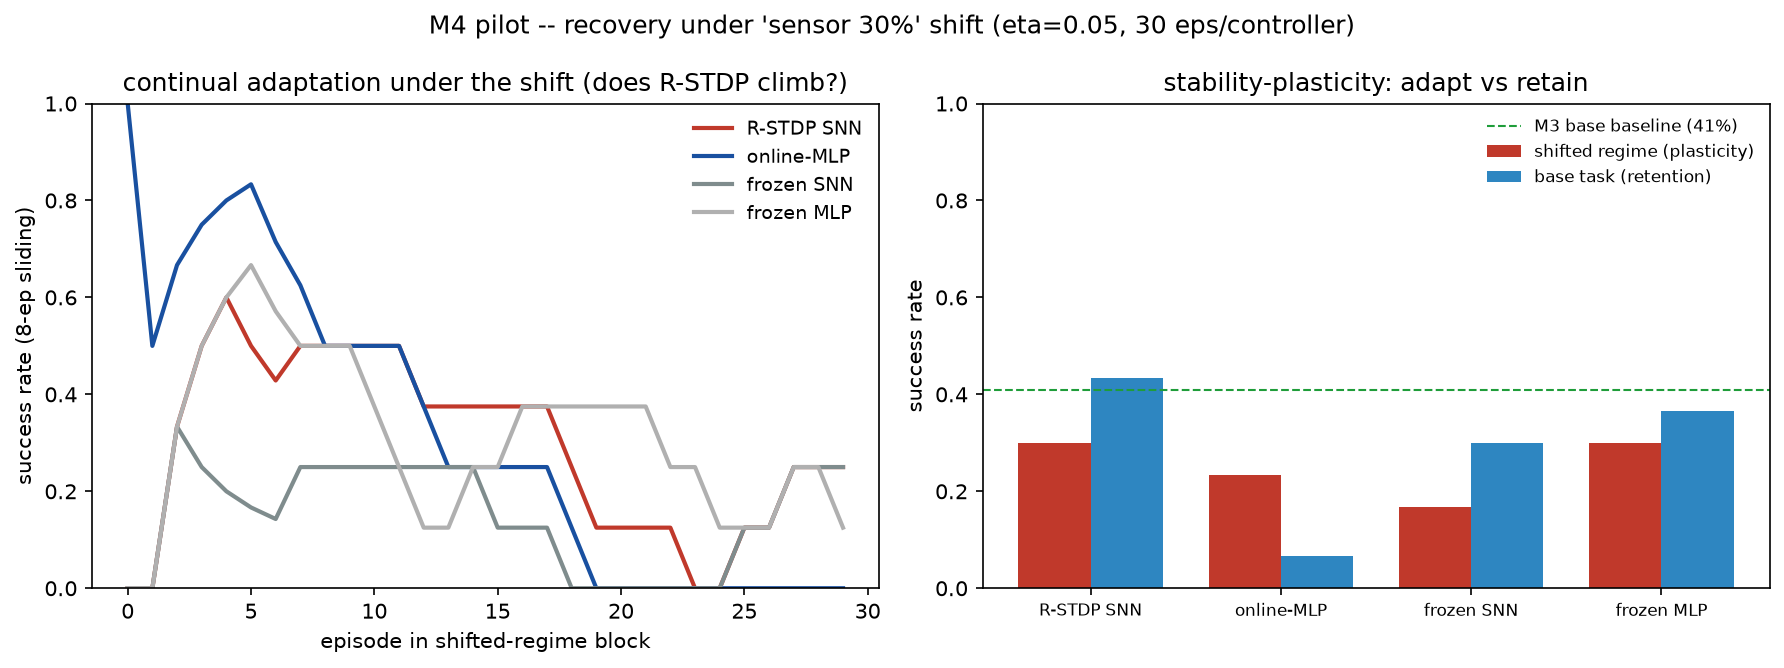
\includegraphics[width=\linewidth]{images/fig_pilot_sensor.png}
\end{column}
\begin{column}{0.36\textwidth}
\begin{tikzpicture}
  \node[fill=navy,rounded corners=6pt,text width=4.3cm,align=left,
        anchor=north west,inner sep=10pt] (b) at (0,0)
    {\footnotesize
     {\bfseries\color{goldcol}Το R-STDP είναι ο ΜΟΝΟΣ ελεγκτής που:}\\[8pt]
     {\color{greencol}\checkmark}{\color{white} προσαρμόζεται στη βλάβη (30\%, ισοβαθμία)}\\[5pt]
     {\color{greencol}\checkmark}{\color{white} ΔΕΝ ξεχνά το αρχικό έργο (43\%, κορυφαίο)}\\[10pt]
     {\itshape\color{ice} Το Online MLP ανέκαμψε αρχικά αλλά κατέρρευσε — ``κατέστρεψε'' τη μνήμη του (7\%).}\\[10pt]
     {\fontsize{8}{9.5}\selectfont\color{goldcol}
      $\triangle$ Στατιστικά: θετικό σήμα, όχι ακόμα απόδειξη (τα CI επικαλύπτονται στα
      n=30). Το M5 το επιβεβαιώνει με $\geq$10 seeds.}
    };
\end{tikzpicture}
\end{column}
\end{columns}
\end{frame}

% ===================================================================
% 8. Πριν & μετά (video stills)
% ===================================================================
\begin{frame}{Στην πράξη: πριν \& μετά}
{\footnotesize\itshape\color{mutedcol}
Πλήρη βίντεο (mp4) στον φάκελο \texttt{videos/}\par}
\vspace{2mm}
\begin{columns}[T]
\begin{column}{0.49\textwidth}
  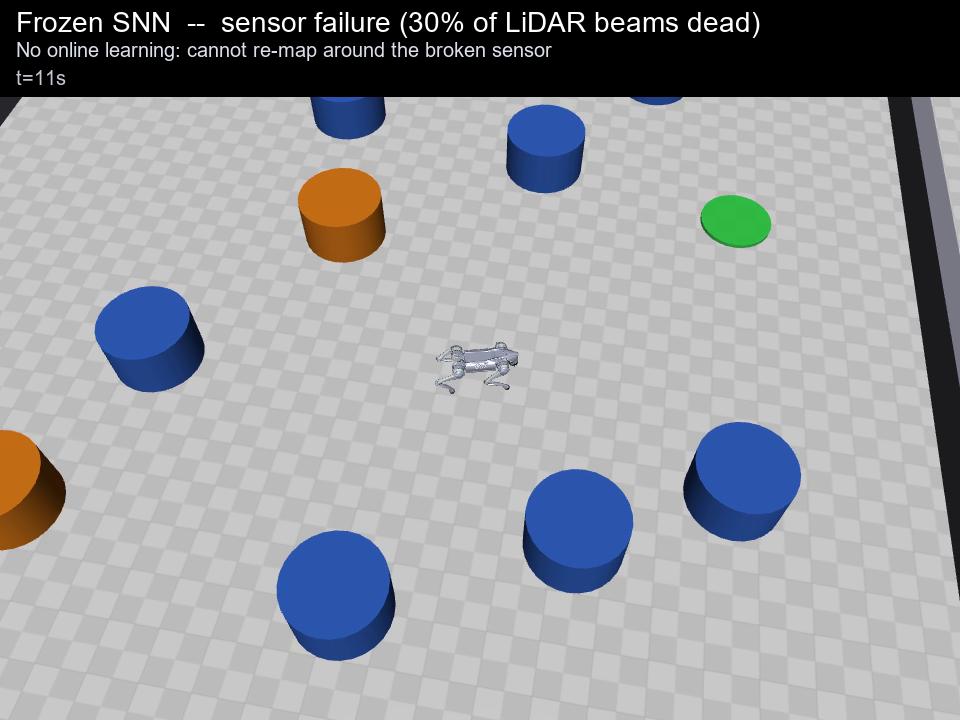
\includegraphics[width=\linewidth]{images/frame_before.png}\\[2mm]
  \begin{tikzpicture}
    \node[fill=redcol,rounded corners=3pt,minimum width=\linewidth,minimum height=0.8cm,
          text=white,font=\bfseries\footnotesize] {ΠΡΙΝ — Παγωμένο SNN (χωρίς μάθηση)};
  \end{tikzpicture}
\end{column}
\begin{column}{0.49\textwidth}
  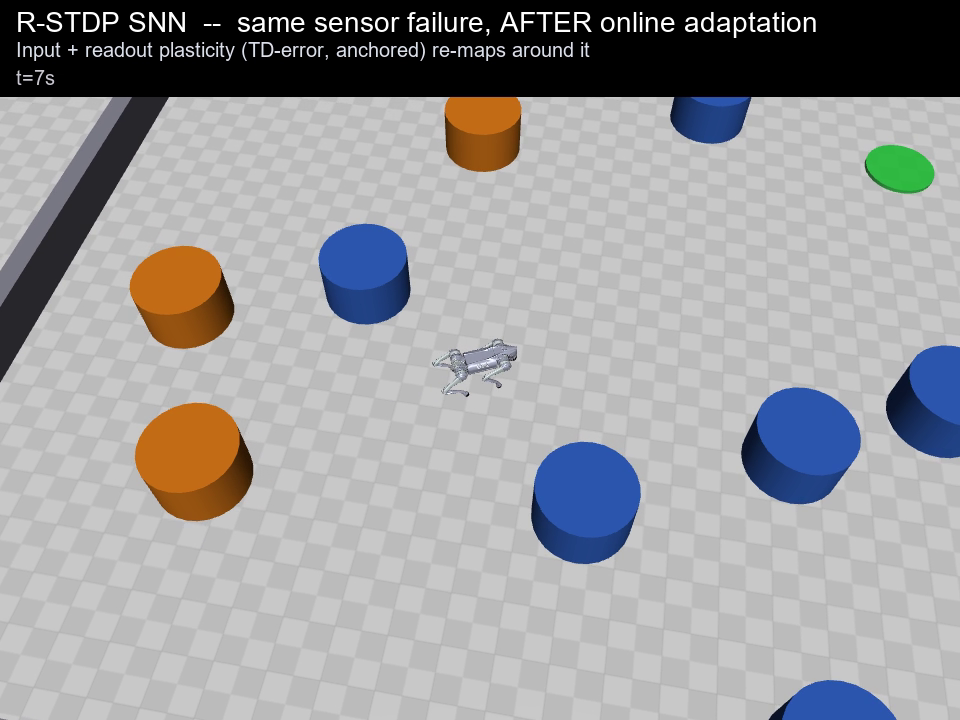
\includegraphics[width=\linewidth]{images/frame_after.png}\\[2mm]
  \begin{tikzpicture}
    \node[fill=greencol,rounded corners=3pt,minimum width=\linewidth,minimum height=0.8cm,
          text=white,font=\bfseries\footnotesize] {ΜΕΤΑ — R-STDP προσαρμοσμένο online};
  \end{tikzpicture}
\end{column}
\end{columns}
\end{frame}

% ===================================================================
% 9. Τι μένει
% ===================================================================
\begin{frame}{Τι μένει}
\begin{tikzpicture}
  \def\cols{%
    0/navy/white/ice/{M5}/{Πλήρης σύγκριση,\\ $\geq$10 seeds}/{στατιστική σημαντικότητα},%
    1/ice/txtcol/mutedcol/{M6}/{Robustness\\ + ενέργεια}/{θόρυβος, SynOps vs MACs},%
    2/ice/txtcol/mutedcol/{M7--M8}/{FPGA\\ υλοποίηση}/{crossbar-inspired επιτάχυνση},%
    3/ice/txtcol/mutedcol/{M9}/{Γράψιμο \&\\ υπεράσπιση}/{διπλωματική εργασία}%
  }
  \foreach \i/\bg/\fg/\dcol/\code/\ttl/\dsc in \cols {
    \pgfmathsetmacro{\x}{\i*3.15}
    \node[fill=\bg,rounded corners=6pt,minimum width=2.9cm,minimum height=4.6cm,anchor=north west]
      (card\i) at (\x,0) {};
    \node[anchor=north,text=\fg,font=\headfont\bfseries\fontsize{18}{18}\selectfont]
      at ($(card\i.north)+(0,-0.55)$) {\code};
    \node[anchor=north,text width=2.55cm,align=center,text=\fg,font=\bfseries\footnotesize]
      at ($(card\i.north)+(0,-1.35)$) {\ttl};
    \node[anchor=north,text width=2.55cm,align=center,
          text=\dcol,font=\fontsize{9}{11}\selectfont]
      at ($(card\i.north)+(0,-2.75)$) {\dsc};
  }
  \node[anchor=north west,text width=11.8cm,align=left,font=\footnotesize\itshape,
        text=mutedcol] at (0,-5.3)
    {Το proposal προβλέπει ακριβώς αυτά τα 5 βήματα (D1--D3 ολοκληρώθηκαν, M1--M4 ολοκληρώθηκαν).};
\end{tikzpicture}
\end{frame}

% ===================================================================
% 10. Κλείσιμο
% ===================================================================
\begin{frame}[plain]
\begin{tikzpicture}[remember picture,overlay]
  \fill[navy] (current page.south west) rectangle (current page.north east);
  \fill[navytwo] ($(current page.north east)+(-2.1,-0.9)$) circle (1.05);
  \fill[goldcol,opacity=0.30] ($(current page.south west)+(1.1,1.1)$) circle (0.8);
  \node[anchor=center] at ($(current page.center)+(0,0.4)$)
    {\headfont\bfseries\fontsize{36}{36}\selectfont\color{white} Ευχαριστώ};
  \node[anchor=center] at ($(current page.center)+(0,-0.5)$)
    {\fontsize{16}{16}\selectfont\color{ice} Ερωτήσεις;};
\end{tikzpicture}
\end{frame}

\end{document}
